% Template LaTeX document for CSSR4Africa Deliverables
% Adapted from documents prepared by EPFL for the RobotCub project
% and subsequently by the University of Skövde for the DREAM project
%
% DV 28/06/2023

\documentclass{CSSRforAfrica}

\usepackage[hidelinks,colorlinks=false]{hyperref}
\usepackage[titletoc,title]{appendix}
\usepackage{latexsym}
% \usepackage{xcolor}
\usepackage{dirtree}
\usepackage[utf8]{inputenc}
\usepackage{listings}

\usepackage{tikz}
\usepackage{amsmath}
\usetikzlibrary{shapes.geometric, arrows, positioning, fit}
\usetikzlibrary{positioning, arrows.meta, calc, fit, backgrounds}

\newcommand{\blank}{~\\}
\newcommand{\checkbox}{{~~~~~~~\leavevmode \put(-7,-1.5){  \huge $\Box$  }}}

\begin{document}
\input{epsf}

%%
%% SHOULD NOT NEED TO BE CHANGED BEFORE THIS POINT
%% ------------------------------------------------
%%

\deliverable{D5.5.2.3}    
\title{D5.5.2.3 Kinyarwanda Text to Speech Conversion}    

\leadpartner{ Carnegie Mellon University Africa} 
\partner{}                                % INSERT partner name: Carnegie Mellon University Africa or The University of the Witwatersrand

\revision{1.2}  
\deliverabledate{26/02/2025} 
\submissiondate{02/03/2025}  
\revisiondate{16/06/2025}   
\disseminationlevel{PU}
\responsible{Richard Muhirwa }     

%%
%% Create the titlepage
%%

\maketitle
 

\section*{Executive Summary}
%===============================================================
\label{executive_summary}
%%\addcontentsline{toc}{section}{Executive Summary} 

Deliverable D5.5.2.3 concerns the results of Task 5.5.2.3, a task whose objective was to train, test, and deploy a text-to-speech (TTS) model for the Kinyarwanda language. This model aims to synthesize natural-sounding speech from text inputs, enabling the generation of audio output.  

This report details the output of each phase of the software development process used in the fulfillment of Deliverable D5.5.2.3. The \textbf{requirements definition} section specifies the functional requirements of KinyarwandaTTS, outlining its role in delivering accurate and natural speech synthesis for Kinyarwanda-speaking users. The \textbf{module specification} section describes the core functionality of the TTS model, including its linguistic alignment and phonetic optimization for the Kinyarwanda language. The \textbf{interface design} section outlines the inputs and outputs of the TTS system, detailing how text inputs are converted into audio streams. The \textbf{module design} section delves into the architecture of the deep learning models employed, focusing on their ability to capture phonetic and prosodic features unique to Kinyarwanda. The \textbf{testing} section showcases the results and descriptions of unit and end-to-end tests conducted to evaluate the accuracy, intelligibility, and naturalness of the synthesized speech. Lastly, the \textbf{user manual} section provides step-by-step instructions on how to deploy and utilize the KinyarwandaTTS model.  


\newpage
 
 
%\graphicspath{{./figs/}}
\pagebreak
\tableofcontents
\newpage


\section{Introduction}
%===============================================================
Text-to-Speech (TTS) systems play a crucial role in enabling natural and effective communication between humans and machines. A TTS system converts written text into spoken speech, serving as the final step in many conversational and assistive technologies. \\

\begin{figure}[h]
    \centering
    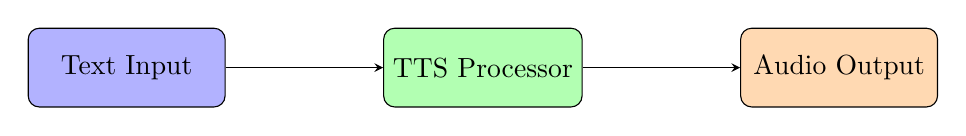
\begin{tikzpicture}[node distance=2cm]
        \node[draw, fill=blue!30, rounded corners, minimum width=2.5cm, minimum height=1cm] (input) {Text Input};
        \node[draw, fill=green!30, rounded corners, minimum width=2.5cm, minimum height=1cm, right=of input] (processor) {TTS Processor};
        \node[draw, fill=orange!30, rounded corners, minimum width=2.5cm, minimum height=1cm, right=of processor] (output) {Audio Output};
        
        \draw[-stealth] (input) -- (processor);
        \draw[-stealth] (processor) -- (output);
    \end{tikzpicture}
    \caption{Basic workflow of a Text-to-Speech system, showing the conversion path from input text through processing to audio output.}
    \label{fig:tts-workflow}
\end{figure}

A TTS system typically consists of several components: text preprocessing, linguistic analysis, prosody generation, and speech synthesis as illustrated in Figure~\ref{fig:tts-workflow}. Text preprocessing involves cleaning and normalizing text inputs, linguistic analysis maps the text to phonetic representations, prosody generation determines the rhythm and intonation of the speech, and speech synthesis produces audio output that conveys the desired naturalness. Together, these components enable TTS systems to generate speech that is both accurate and contextually appropriate.

The KinyarwandaTTS module developed in this deliverable focuses exclusively on the text-to-speech component. It is designed to synthesize speech in Kinyarwanda. The model receives text inputs, processes them to capture linguistic and phonetic nuances unique to Kinyarwanda, and produces natural-sounding audio outputs.

This development is part of a broader initiative to create culturally sensitive social robotics applications for African contexts, where the ability to communicate in local languages is essential for acceptance and effectiveness. By enabling robots to speak Kinyarwanda naturally, we aim to make human-robot interaction more intuitive and accessible for Kinyarwanda speakers, supporting applications in education, healthcare, customer service, and other domains where voice interaction is valuable.

 
\newpage
\section{Requirements Definition}
%===============================================================

A running \textbf{KinyarwandaTTS} system performs one main function—converting Kinyarwanda text input into natural-sounding speech. The system receives text inputs, processes the text to account for Kinyarwanda-specific linguistic and phonetic rules, and generates corresponding audio outputs that capture the rhythm, intonation, and natural flow of the language.  

In order to feasibly perform this function, the following functional requirements need to be fulfilled by \textbf{KinyarwandaTTS}:  

\begin{enumerate}

\item \textbf{Input Text Parsing and Preprocessing}  
   - Receive Kinyarwanda text input in UTF-8 format through an accessible interface (e.g., file input, or command-line argument).  
   - Normalize the text by removing unnecessary symbols, handling punctuation, and resolving abbreviations to ensure proper pronunciation.  

\item \textbf{Phonetic and Linguistic Analysis}  
   - Map the normalized text to phonetic representations tailored to Kinyarwanda's unique linguistic structure.  
   - Generate prosody features, such as pitch, duration, and stress patterns, to mimic the natural intonation and rhythm of spoken Kinyarwanda.  

\item \textbf{Speech Synthesis}
   - Use a trained deep learning-based TTS model to synthesize high-quality audio output from the processed text and prosody features.  
   - Ensure the audio output is natural-sounding, with minimal artifacts.  

\item \textbf{Output Speech Generation}  
   - Generate and deliver the synthesized speech as an audio file in standard formats (e.g., WAV, MP3).  
   - Provide the option to output the audio stream directly for real-time playback.  



\end{enumerate}


\newpage
\section{Module Specification}
%===============================================================
The KinyarwandaTTS module is responsible for converting text messages into synthesized speech in the Kinyarwanda language and playing the generated audio on a remote robot, such as Pepper. The module is implemented as a ROS node that interacts with other ROS topics and external systems. Below are the detailed specifications of the module:

\subsection{Functional Characteristics}

\subsubsection{Text-to-Speech Conversion}
\begin{itemize}
    \item The core functionality of the module is to synthesize  Kinyarwanda speech 
    from text received on the 
%%\colorbox{lightgray}{\texttt{/text\_to\_say}} 
\texttt{/text\_to\_say}
ROS topic.
    \item The Coqui TTS is a free text-to-speech (TTS) library that uses deep learning to convert text to audio. Coqui TTS model is used for generating speech, with pre-trained models and 
    configuration files specified during initialization.
\end{itemize}

\subsubsection{Audio File Generation}
The synthesized speech is saved as a temporary \texttt{.wav} audio file for playback. The temporary file is created using Python's \texttt{tempfile} library and deleted automatically after playback.

\subsubsection{Audio Playback on Remote Robot}
The module uses the \texttt{send\_and\_play\_audio.py} script to transmit the audio file to the robot and play it. Secure transfer of the audio file is achieved using \texttt{sshpass} and \texttt{scp}. Playback is managed by the NAOqi framework via the \texttt{ALAudioPlayer} proxy on the robot.

\subsubsection{ROS Integration}
The ROS node subscribes to the \texttt{/text\_to\_say} topic of type \texttt{std\_msgs/String}, receiving text messages to convert to speech. It can be launched using the \texttt{rosrun} command from a properly set-up ROS workspace.

\subsection{Inputs and Outputs}

\subsubsection{Inputs}
\begin{itemize}
    \item \textbf{ROS Topic:} \texttt{/text\_to\_say}
    \begin{itemize}
        \item \textbf{Type:} \texttt{std\_msgs/String}
        \item \textbf{Description:} Accepts a text string in Kinyarwanda to be converted into speech.
    \end{itemize}
\end{itemize}

\subsubsection{Outputs}
\begin{itemize}
    \item \textbf{Audio File:} A temporary \texttt{.wav} file generated during runtime and used for playback.
    \item \textbf{Remote Playback:} The synthesized speech is played back on the robot via the NAOqi framework.
\end{itemize}

\subsection{Dependencies}

\subsubsection{Python Dependencies}
\begin{itemize}
    \item \texttt{rospy} (ROS integration)
    \item \texttt{std\_msgs} (ROS message types)
    \item \texttt{tempfile} (temporary file handling)
    \item \texttt{subprocess} (external process execution)
    \item \texttt{os} (file system operations)
    \item Coqui TTS (\texttt{TTS.utils.synthesizer.Synthesizer})
\end{itemize}

\subsubsection{NAOqi Framework}
\begin{itemize}
    \item \texttt{ALProxy} (audio playback proxy)
    \item Secure communication and file transfer using \texttt{sshpass} and \texttt{scp}.
\end{itemize}

\subsubsection{External Files}
\begin{itemize}
    \item Model files for TTS, including \texttt{.pth} and \texttt{.json} configurations, located in\\ \texttt{\$HOME/tts\_ws/src/kinyarwanda\_tts/model\_files/}.
    \item \texttt{send\_and\_play\_audio.py} script for transferring and playing the audio on the robot.
\end{itemize}

\subsection{Configuration}

The module requires the following configurations for proper operation:
\begin{itemize}
    \item \textbf{TTS Model Paths:} Paths to pre-trained TTS model files (\texttt{model.pth}, \texttt{config.json}, etc.).
    \item \textbf{Python Version:} The primary ROS node runs on Python 3.9, while the playback script uses Python 2.
    \item \textbf{Robot Connection:}
    \begin{itemize}
        \item \textbf{Robot's IP address:} \texttt{172.29.111.230}.
        \item \textbf{Robot's username:} \texttt{nao}.
        \item \textbf{Robot's password:} \texttt{nao}.
    \end{itemize}
\end{itemize}

\subsection{Execution Workflow}

\subsubsection{Node Initialization}
The ROS node \texttt{kinyarwandaTTS} initializes and sets up the Coqui TTS synthesizer. The \texttt{/text\_to\_say} topic subscriber is registered.

\subsubsection{Text Reception}
The node receives text input via the \texttt{/text\_to\_say} topic.

\subsubsection{Speech Synthesis}
The received text is processed and converted into a \texttt{.wav} audio file using the TTS model.

\subsubsection{Audio Playback}
The generated audio file is securely transferred to the robot. The playback script (\texttt{send\_and\_play\_audio.py}) executes the file on the robot and deletes it after playback.

\subsection{System Requirements}
\begin{itemize}
    \item ROS workspace configured with the NAOqi drivers.
    \item Coqui TTS model and required dependencies installed.
    \item Python 3.9 for the ROS node and Python 2 for the playback script.
    \item SSH connection between the local system and the robot.
\end{itemize}

\subsection{Limitations and Assumptions}

    The current implementation assumes that the robot (e.g., Pepper) is accessible over SSH and correctly configured with NAOqi drivers.
    The playback script must be compatible with the target robot's operating environment.
    Temporary .wav files must be generated and deleted properly to avoid storage issues.



\newpage
\section{Interface Design}
%===============================================================
\subsection{Directory Structure}

The directory structure of the \texttt{kinyarwanda\_tts} module is as follows:

\vspace{1cm}

\dirtree{%
.1 cssr4africa/.
.2 cssr\_system/.
.3 kinyarwanda\_tts/.
.4 launch/.
.4 model\_files/.
.5 conditioning\_audio.wav.
.5 conditioning\_audio2.wav.
.5 config\_se.json.
.5 config.json.
.5 model.pth.
.5 README.md.
.5 SE\_checkpoint.pth.tar.
.5 speakers.pth.
.4 src/.
.5 send\_and\_play\_audio.py.
.5 kinyarwanda\_tts\_node.py.
.3 README.md.
.3 package.xml.
.3 CMakeLists.txt.
.2 unit\_test/.
.3 ....
}
\vspace{1cm}

\textbf{Explanation of File and Folder Structure}
\begin{enumerate}

    \item \colorbox{lightgray}{\texttt{launch/}}
    \begin{itemize}
        \item Contains the launch file for starting the KinyarwandaTTS ROS node.
    \end{itemize}
    
    \item \colorbox{lightgray}{\texttt{model\_files/}}
    \begin{itemize}
        \item Stores the TTS model files and configurations:
        \begin{itemize}
            \item model.pth: Pre-trained Coqui TTS model.
            \item config.json: Configuration file for the TTS model.
            \item speakers.pth: Speaker embeddings for voice customization.
            \item SE\_checkpoint.pth.tar: Speaker encoder checkpoint file.
            \item config\_se.json: Configuration file for the speaker encoder.
            \item conditioning\_audio.wav: Audio file for conditioning the model.
        \end{itemize}
    \end{itemize}

\newpage
% ============================================================================================
    \item \colorbox{lightgray}{\texttt{scripts/}}
    \begin{itemize}
        \item Contains additional scripts used by the node:
        \begin{itemize}
            \item \texttt{send\_and\_play\_audio.py}: Python 2 script to transfer and play audio on the robot.
            \item \texttt{\_\_init\_\_.py}: Marks the directory as a Python module.
        \end{itemize}
    \end{itemize}
    
    \item \colorbox{lightgray}{\texttt{src/}}
    \begin{itemize}
        \item Contains the main source code for the KinyarwandaTTS ROS node:
        \begin{itemize}
            \item \texttt{tts\_node.py}: Core Python script implementing the node functionality.
        \end{itemize}
    \end{itemize}
    
    \item \colorbox{lightgray}{\texttt{tests/}}
    \begin{itemize}
        \item Contains unit tests and integration tests for the node:
        \begin{itemize}
            \item \texttt{test\_tts\_node.py}: Test suite for validating the TTS functionality.
            \item \texttt{\_\_init\_\_.py}: Marks the directory as a Python module.
        \end{itemize}
    \end{itemize}
    
    \item \textbf{Root Files}
    \begin{itemize}
        \item \texttt{README.md}: Documentation file with instructions on setup and usage.
        \item \texttt{package.xml}: ROS package metadata.
        \item \texttt{CMakeLists.txt}: Build configuration for the ROS package.
        \item \texttt{requirements.txt}: Python dependencies required for the node.
    \end{itemize}    
\end{enumerate}


\newpage
\section{Module Design}
%===============================================================

The module design of the KinyarwandaTTS system implements an end-to-end architecture for text-to-speech synthesis for the Kinyarwanda language, as shown in the \ref{Inference procedure}. The system follows a unified pipeline based on a conditional variational autoencoder with adversarial learning.


\subsection {Text Encoding and Prior Encoder}

This component processes input text and language information to create the foundation for speech synthesis. The prior encoder processes input text through character embedding and incorporates language ID information via language embedding. These embeddings are then transformed through a transformer-based encoder with relative positional representation instead of absolute positional encoding. A linear projection layer produces the mean and variance for constructing the prior distribution. The architecture includes a stack of affine coupling layers consisting of WaveNet residual blocks for normalizing flow, using volume-preserving transformation with Jacobian determinant of one for simplicity\cite{kim2021conditional}.


\subsection {Neural Acoustic Modeling with Stochastic Duration Prediction}

This component transforms text representations into acoustic features through interconnected neural network components. The system generates hidden text representation (htext) via the transformer encoder and predicts phoneme duration distributions through the stochastic duration predictor. It creates alignment information through linear projection and applies flow-based decoding with affine coupling layers. The stochastic duration predictor utilizes residual blocks with dilated and depth-separable convolutional layers, along with neural spline flows for improved transformation expressiveness in coupling layers. The component integrates speaker embedding from reference audio with global conditioning and supports noise input to enable variability in synthesis \cite{kim2021conditional}.


%\newpage
% ===============================================================================
\subsection {HiFi-GAN Decoder for Waveform Generation}

This component converts the acoustic features into the final audio waveform using a high-fidelity neural vocoder. The HiFi-GAN decoder generates high-fidelity speech waveforms from the flow-based decoder output and applies transposed convolutions followed by multi-receptive field fusion modules (MRF). It follows the HiFi-GAN V1 generator architecture with stacked transposed convolutions, and the multi-receptive field fusion modules combine residual blocks with different receptive field sizes. A linear transformation of speaker embedding is added to the input latent variables (z), enabling high-quality audio synthesis that preserves the linguistic nuances of Kinyarwanda \cite{kim2021conditional}.

\subsection {Speech Synthesis Module}

This is the runtime module where the actual speech synthesis takes place using the trained end-to-end model. The module orchestrates the complete inference pipeline from text to speech and converts text input into audio waveforms following the procedure in the diagram. It utilizes the pre-trained end-to-end conditional variational autoencoder model and supports GPU acceleration for faster synthesis when available. During inference, the system omits the posterior encoder and discriminator components that are only used during the training phase. The module accepts raw text in Kinyarwanda and optional reference audio for speaker characteristics as inputs, and produces raw audio waveform in .wav format as its output.
See Figure \ref{Training procedure} and Figure \ref{Inference procedure} for training and inference procedures.
%========================================================================

\begin{figure}

\usetikzlibrary{shapes,arrows,positioning,fit,backgrounds}

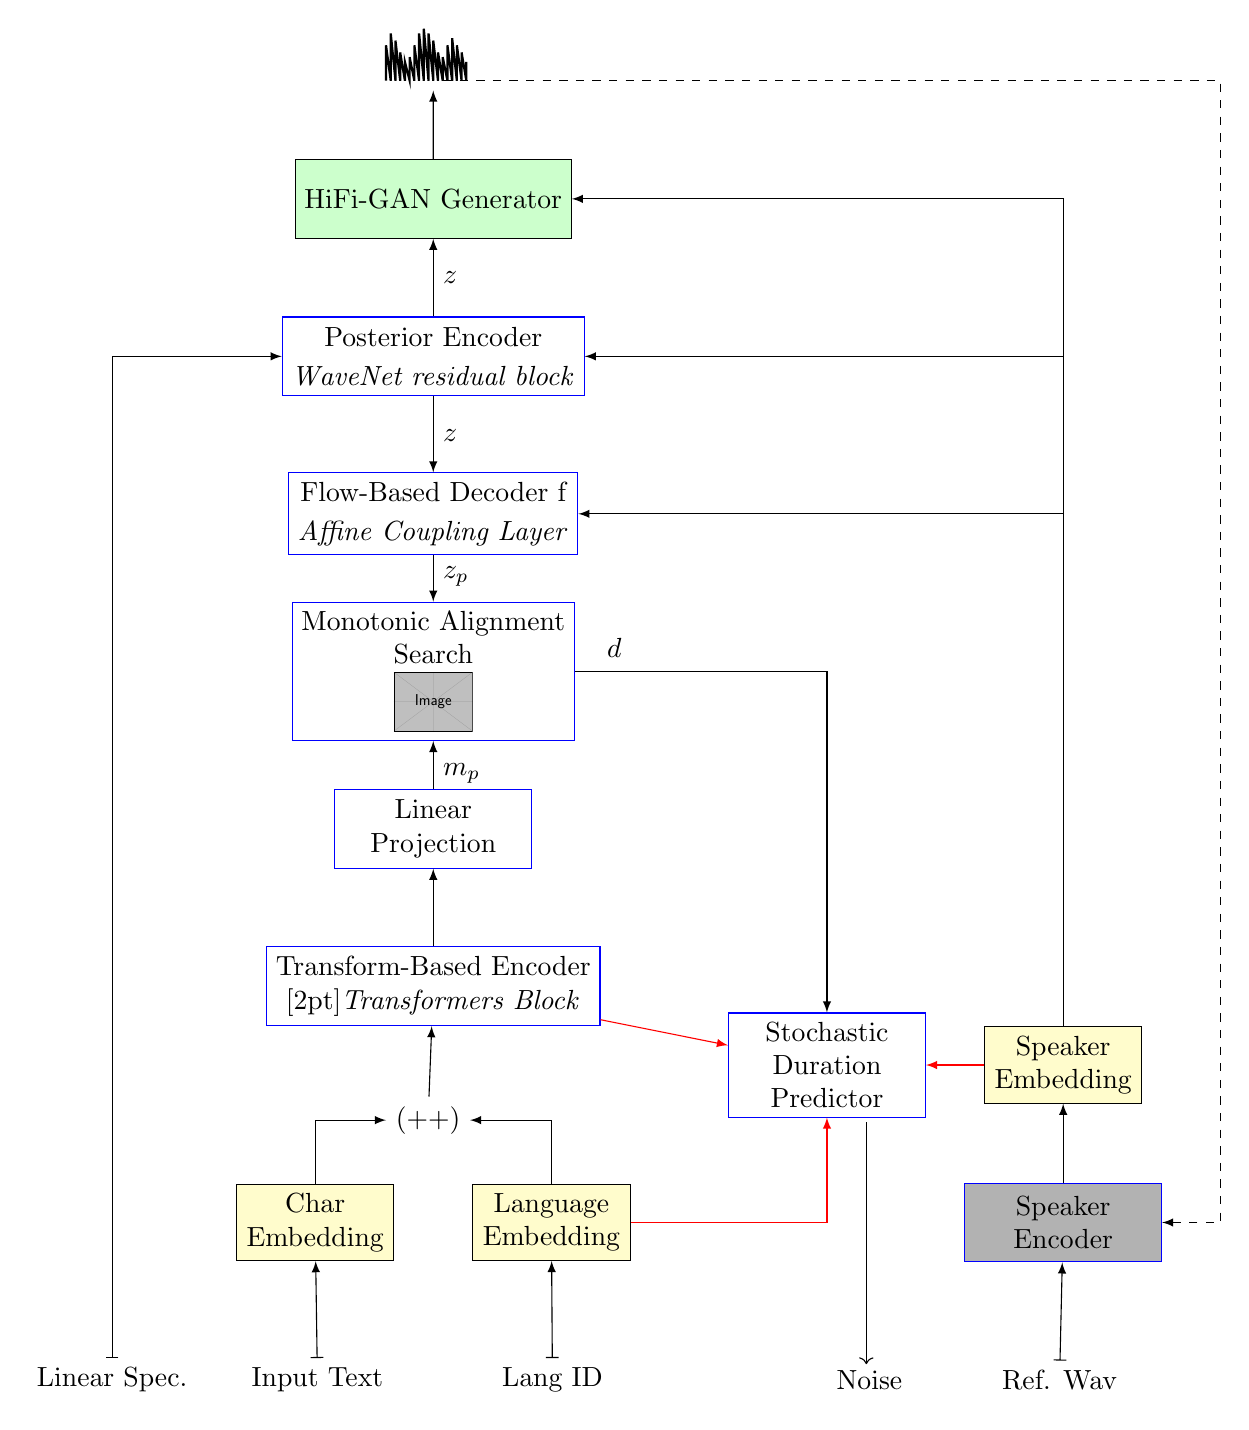
\begin{tikzpicture}[
    box/.style={draw=blue, fill=white, minimum width=2.5cm, minimum height=1cm, align=center},
    greenbox/.style={draw=black, fill=green!20, minimum width=2.5cm, minimum height=1cm, align=center},
    smallbox/.style={draw=black, fill=yellow!20, minimum width=2cm, minimum height=0.6cm, align=center},
    dotted/.style={draw=orange, dotted, thick},
    arrow/.style={->, >=latex}, arrow2/.style={<-, >=latex}, 
    arrow3/.style={|->, >=latex}
]

\begin{scope}[scale=0.3]
        \node (sound) at (10,45) {}; % Define the node
        \draw[thick] (8,45)
            -- ++(0,1.5) -- ++(0.2,-1.5) -- ++(0,2)   -- ++(0.2,-2)   -- ++(0,1.7)
            -- ++(0.2,-1.7) -- ++(0,1.2) -- ++(0.2,-1.2) -- ++(0,0.8) -- ++(0.2,-0.8)
            -- ++(0,1) -- ++(0.2,-1) -- ++(0,1.5) -- ++(0.2,-1.5) -- ++(0,2)
            -- ++(0.2,-2) -- ++(0,2.2) -- ++(0.2,-2.2) -- ++(0,2) -- ++(0.2,-2)
            -- ++(0,1.7) -- ++(0.2,-1.7) -- ++(0,1.2) -- ++(0.2,-1.2) -- ++(0,1)
            -- ++(0.2,-1) -- ++(0,1.5) -- ++(0.2,-1.5) -- ++(0,1.8) -- ++(0.2,-1.8)
            -- ++(0,1.5) -- ++(0.2,-1.5) -- ++(0,1.2) -- ++(0.2,-1.2) -- ++(0,0.8);
\end{scope}

% Input elements at the bottom
\node[left] (spec) at (0,-3) {Linear Spec.};
\node[right] (add) at (2.4,0.3) {$(++)$}; %(++) sign
\node[smallbox] (char) at (1.5,-1) {Char\\ Embedding};
\node[smallbox] (lang) at (4.5,-1) {Language\\ Embedding};
\node[right] (langid) at (3.75,-3) {Lang ID};
\node[right] (in) at (0.57,-3) {Input Text};
\node[right] (no) at (8,-3) {Noise};
\node[right] (ref) at (10.1,-3) {Ref. Wav};

% Main network components
\node[box] (transform) at (3,2) {Transform-Based Encoder\\
    
[2pt]\textit{Transformers Block}};
\node[box] (linear) at (3,4) {Linear\\ Projection};
\node[box] (monotonic) at (3,6) {Monotonic Alignment\\ Search\\[2pt]
    \includegraphics[width=1cm]{example-image}}; % Placeholder for the search visualization
\node[box] (flow) at (3,8) {Flow-Based Decoder f\\[2pt]\textit{Affine Coupling Layer}};
\node[box] (wavenet) at (3,10) {Posterior Encoder\\[2pt]\textit{WaveNet residual block}};
\node[greenbox] (hifi) at (3,12) {HiFi-GAN Generator};

% Side components
\node[box] (stochastic) at (8,1) {Stochastic\\ Duration\\ Predictor};
\node[smallbox] (speaker1) at (11,1) {Speaker\\ Embedding};
\node[box, fill=gray!60] (speaker2) at (11,-1) {Speaker\\ Encoder};

% Draw arrows
% \draw[arrow] (spec) -- (transform);
\draw[arrow] (hifi) -- (sound);
\draw[arrow3] (in) -- (char);
\draw[arrow3] (langid) -- (lang);
\draw[arrow] (transform) -- (linear);
\draw[arrow] (linear) -- (monotonic);
\draw[arrow2] (monotonic) -- (flow);
\draw[arrow2] (flow) -- (wavenet);
\draw[arrow] (wavenet) -- (hifi);
\draw[red,arrow] (transform) -- (stochastic);
\draw[arrow3] (ref) -- (speaker2);
\draw[arrow] (speaker2) -- (speaker1);
\draw [->] (8.5,0.27) -- (8.5,-2.8);
\draw[red,arrow] (speaker1) -- (stochastic);
\draw[arrow] (add) -- (transform);

% Side connections
\draw[arrow2] (stochastic) |- (monotonic);
\draw[arrow] (speaker1) |- (hifi);
\draw[arrow] (speaker1) |- (flow);
\draw[arrow] (speaker1) |- (wavenet);
\draw[arrow3] (spec) |- (wavenet);
\draw[red,arrow] (lang) -| (stochastic);
\draw[dashed, arrow] (sound) -| (13,-1) -- (speaker2);
\draw[arrow] (lang) |- (add);
\draw[arrow] (char) |- (add);

% Add orange dotted boxes
%\node[dotted, fit=(wavenet)] {};
%\node[dotted, fit=(transform)] {};
%\node[dotted, fit=(flow)] {};

% Add variables
\node[right] at (3,11) {$z$};
\node[right] at (3,9) {$z$};
\node[right] at (3,7.2) {$z_p$};
\node[right] at (3,4.7) {$m_p$};
\node at (5.3,6.3) {$d$};


\end{tikzpicture}
\caption{Kinyarwanda TTS training procedure showing the data flow between text encoder, flow-based decoder, and audio generation components. \cite{casanova2022yourtts}} 
\label{Training procedure}
\end{figure}

%======================================================================
\begin{figure}

\usetikzlibrary{shapes,arrows,positioning,fit,backgrounds}

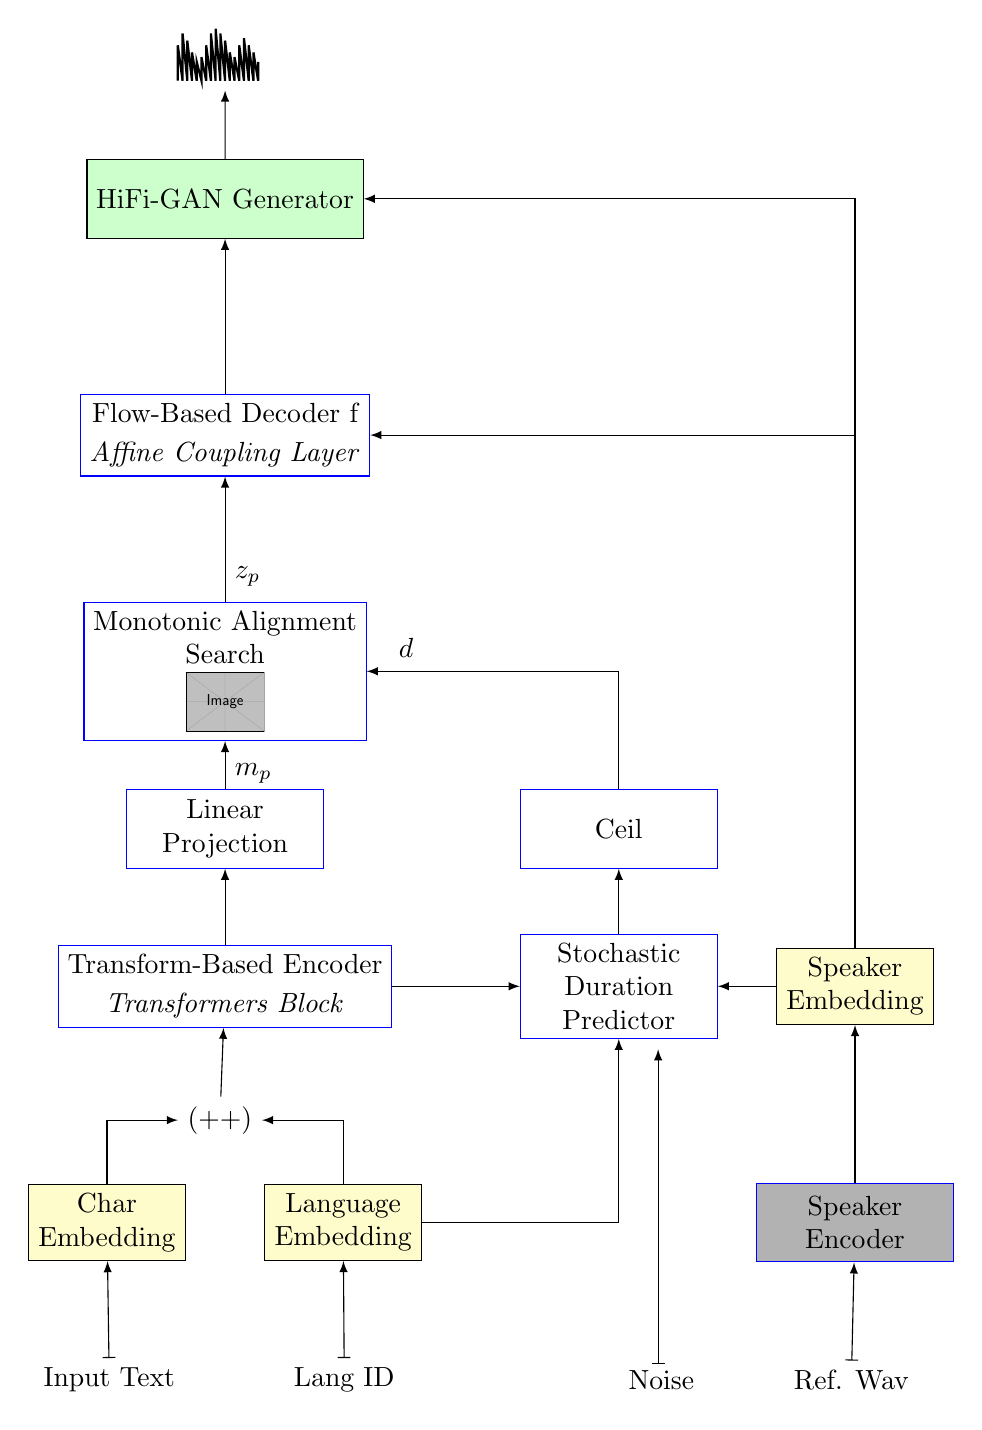
\begin{tikzpicture}[
    box/.style={draw=blue, fill=white, minimum width=2.5cm, minimum height=1cm, align=center},
    greenbox/.style={draw=black, fill=green!20, minimum width=2.5cm, minimum height=1cm, align=center},
    smallbox/.style={draw=black, fill=yellow!20, minimum width=2cm, minimum height=0.6cm, align=center},
    dotted/.style={draw=orange, dotted, thick},
    arrow/.style={->, >=latex}, arrow2/.style={<-, >=latex}, 
    arrow3/.style={|->, >=latex}
]

\begin{scope}[scale=0.3]
        \node (sound) at (10,45) {}; % Define the node
        \draw[thick] (8,45)
            -- ++(0,1.5) -- ++(0.2,-1.5) -- ++(0,2)   -- ++(0.2,-2)   -- ++(0,1.7)
            -- ++(0.2,-1.7) -- ++(0,1.2) -- ++(0.2,-1.2) -- ++(0,0.8) -- ++(0.2,-0.8)
            -- ++(0,1) -- ++(0.2,-1) -- ++(0,1.5) -- ++(0.2,-1.5) -- ++(0,2)
            -- ++(0.2,-2) -- ++(0,2.2) -- ++(0.2,-2.2) -- ++(0,2) -- ++(0.2,-2)
            -- ++(0,1.7) -- ++(0.2,-1.7) -- ++(0,1.2) -- ++(0.2,-1.2) -- ++(0,1)
            -- ++(0.2,-1) -- ++(0,1.5) -- ++(0.2,-1.5) -- ++(0,1.8) -- ++(0.2,-1.8)
            -- ++(0,1.5) -- ++(0.2,-1.5) -- ++(0,1.2) -- ++(0.2,-1.2) -- ++(0,0.8);
\end{scope}

% Input elements at the bottom
%\node[left] (spec) at (0,-3) {Linear Spec.};

\node[right] (add) at (2.4,0.3) {$(++)$}; %(++) sign
\node[smallbox] (char) at (1.5,-1) {Char\\ Embedding};
\node[smallbox] (lang) at (4.5,-1) {Language\\ Embedding};
\node[right] (langid) at (3.75,-3) {Lang ID};
\node[right] (in) at (0.57,-3) {Input Text};
\node[right] (no) at (8,-3) {Noise};
\node[right] (ref) at (10.1,-3) {Ref. Wav};

% Main network components
\node[box] (transform) at (3,2) {Transform-Based Encoder\\
    [2pt]\textit{Transformers Block}};
    
\node[box] (linear) at (3,4) {Linear\\ Projection};
\node[box] (monotonic) at (3,6) {Monotonic Alignment\\ Search\\[2pt]
    \includegraphics[width=1cm]{example-image}}; % Placeholder for the search visualization
\node[box] (flow) at (3,9) {Flow-Based Decoder f\\[2pt]\textit{Affine Coupling Layer}};
% \node[box] (wavenet) at (3,10) {Posterior Encoder\\[2pt]\textit{WaveNet residual block}};
\node[greenbox] (hifi) at (3,12) {HiFi-GAN Generator};

% Side components
\node[box] (ceil) at (8,4) {Ceil};
\node[box] (stochastic) at (8,2) {Stochastic\\ Duration\\ Predictor};
\node[smallbox] (speaker1) at (11,2) {Speaker\\ Embedding};
\node[box, fill=gray!60] (speaker2) at (11,-1) {Speaker\\ Encoder};


% Draw arrows
% \draw[arrow] (spec) -- (transform);
\draw[arrow] (hifi) -- (sound);
\draw[arrow3] (in) -- (char);
\draw[arrow3] (langid) -- (lang);
\draw[arrow] (transform) -- (linear);
\draw[arrow] (linear) -- (monotonic);
\draw[arrow] (monotonic) -- (flow);
   % \draw[arrow2] (flow) -- (wavenet);
\draw[arrow] (flow) -- (hifi);
\draw[arrow] (transform) -- (stochastic);
\draw[arrow3] (ref) -- (speaker2);
\draw[arrow] (speaker2) -- (speaker1);
\draw[arrow3] (8.5,-2.8) -- (8.5,1.2); %noise
\draw[arrow] (speaker1) -- (stochastic);
\draw[arrow] (stochastic) -- (ceil);
\draw[arrow] (add) -- (transform);

% Side connections
\draw[arrow] (ceil) |- (monotonic);
\draw[arrow] (speaker1) |- (hifi);
\draw[arrow] (speaker1) |- (flow);
%\draw[arrow] (speaker1) |- (wavenet);
%\draw[arrow3] (spec) |- (wavenet);
\draw[arrow] (lang) -| (stochastic);
%\draw[dashed, arrow] (sound) -| (13,-1) -- (speaker2);
\draw[arrow] (lang) |- (add);
\draw[arrow] (char) |- (add);



% Add orange dotted boxes
%\node[dotted, fit=(wavenet)] {};
%\node[dotted, fit=(transform)] {};
%\node[dotted, fit=(flow)] {};

% Add variables
% \node[right] at (3,11) {$z$};
% \node[right] at (3,9) {$z$};
\node[right] at (3,7.2) {$z_p$};
\node[right] at (3,4.7) {$m_p$};
\node at (5.3,6.3) {$d$};


\end{tikzpicture}

\caption{ Kinyarwanda TTS inference procedure depicting how input text is processed and transformed into speech output.
\cite{casanova2022yourtts}}
\label{Inference procedure}
\end{figure}
\newpage
%========================================================================

\subsection {Output Audio Management Module}

This module handles the generated audio output, ensuring proper storage, playback, and streaming capabilities.
\\~\\
\textbf{Responsibilities:}
\begin{itemize}
    \item Save the synthesized audio to a specified file format (e.g., .wav, .mp3).
    \item Provide APIs for real-time audio playback or streaming.
    \item Perform post-processing, such as normalization and noise reduction.
\end{itemize}

\textbf{Key Features:}
\begin{itemize}
    \item Integration with remote systems or robots for audio playback.
    \item Temporary file management for efficient resource utilization.
\end{itemize}


\newpage
%==============================================================

\section{User Manual}

%% This is for code formating {it specifies the background colors, the font to be used and the comments colors}

% Define colors
\definecolor{commentgreen}{RGB}{0, 155, 0}
\definecolor{backgroundcolor}{RGB}{240, 240, 249}
\definecolor{codeblack}{RGB}{0, 0, 0}
% \definecolor{stringblue}{RGB}{255, 165, 0}

% Configure listing style
\lstdefinestyle{commandstyle}{
  backgroundcolor=\color{backgroundcolor},
  basicstyle=\ttfamily\color{codeblack}\footnotesize,
  commentstyle=\color{commentgreen},
  % stringstyle=\color{stringblue},
  numbers=none,
  breaklines=true,
  breakatwhitespace=true,
  tabsize=2,
  showspaces=false,
  showstringspaces=false,
  frame=single,
  framesep=3pt,
  xleftmargin=5pt,
  xrightmargin=5pt,
  framexleftmargin=5pt,
  framexrightmargin=5pt,
  framextopmargin=3pt,
  framexbottommargin=3pt,
  framerule=0pt,
  % The important addition:
  morecomment=[l]{\#},  % This tells LaTeX that lines starting with # are comments
 morestring=[b]',      % Single-quoted strings
 morestring=[b]"       % Double-quoted strings
}


\subsection{Setting Up and Running KinyarwandaTTS}

The KinyarwandaTTS system is implemented as a ROS node that integrates with NAOqi Framework for robotic applications. Follow these steps to set up and run the system:

\subsubsection{Environment Setup}
\begin{enumerate}
    \item Navigate to the root of your ROS workspace:
    \begin{lstlisting}[style=commandstyle]
    cd /your_ros_workspace
    \end{lstlisting}
    \item Compile the ROS packages:
    \begin{lstlisting}[style=commandstyle]
    catkin_make
    \end{lstlisting}
    \item Source the setup file to ensure the environment variables are properly configured:
    \begin{lstlisting}[style=commandstyle]
    source devel/setup.bash
    \end{lstlisting}
\end{enumerate}

\subsubsection{Launching the NAOqi Driver}
Before running the KinyarwandaTTS node, you must establish communication with the robot:

\begin{enumerate}
    \item Launch the NAOqi driver, specifying the robot's IP address and your network interface:
    \begin{lstlisting}[style=commandstyle]
    roslaunch naoqi_driver naoqi_driver.launch 
    nao_ip:=172.29.111.230 network_interface:=enp0s3
    \end{lstlisting}

    \textit{Note: Replace enp0s3 with your actual network interface name if different.}
\end{enumerate}

\subsubsection{Running the KinyarwandaTTS Node}
\begin{enumerate}
    \item Open a new terminal tab or window
    
    \item Source the setup file again in the new terminal:
    \begin{lstlisting}[style=commandstyle]
    source devel/setup.bash
    \end{lstlisting}
    
    \item Launch the KinyarwandaTTS node:
    \begin{lstlisting}[style=commandstyle]
    rosrun kinyarwanda_tts tts_node.py
    \end{lstlisting}
\end{enumerate}

\subsubsection{Testing the System}
To test the TTS functionality, open a third terminal and publish a text message to the \texttt{/text\_to\_say} topic:

\begin{enumerate}
    \item For a simple greeting in Kinyarwanda:
    \begin{lstlisting}[style=commandstyle]
    rostopic pub /text_to_say std_msgs/String "data: 'Mwiriwe neza.'"
    \end{lstlisting}
    
\end{enumerate}

\subsubsection{Troubleshooting}
\begin{itemize}
    \item Ensure the robot is powered on and connected to the same network as your computer
    \item Verify that NAOqi services are running on the robot
    \item Check network connectivity with \texttt{ping 172.29.111.230}
    \item Review ROS logs for error messages: \texttt{rosrun rqt\_console rqt\_console}
\end{itemize}


\newpage
%========================================================================

% Section heading for the unit tests
\section{Kinyarwanda TTS Unit Tests}
% Introduction to the unit tests
This package contains unit tests for the Kinyarwanda Text-to-Speech (TTS) component for Pepper robots.

% Overview subsection with description of the component
\subsection{Overview}
The Kinyarwanda TTS component converts text in Kinyarwanda language to speech and plays it on the Pepper robot. This package provides two primary testing frameworks:
\begin{enumerate}
    \item Standard Test Suite
    \item Interactive Test Mode
\end{enumerate}

% Requirements for running the tests
\subsection{Requirements}
\begin{itemize}
    \item ROS Noetic on Ubuntu 20.04
    \item Python 3.9 (for the TTS node)
    \item Python 2.7 (for the Pepper robot interface)
    \item Coqui TTS library
    \item NAOqi SDK
    \item Local audio playback capability for testing
\end{itemize}

% Detailed explanation of the test harness
\subsection{Test Harness}
% Description of the test harness initialization
\subsubsection{Initialization}
The test harness initializes a connection to the Kinyarwanda TTS node and verifies that the node is running with local playback enabled. The system displays the following banner during initialization:

% Code block showing the banner using verbatim environment
\begin{lstlisting}[style=commandstyle]
======================================================================
KINYARWANDA TTS TEST HARNESS
======================================================================
This harness sends text to the TTS node
Make sure the Kinyarwanda TTS node is running with local playback enabled
Kinyarwanda TTS Test Harness initialized
This harness will send text to the TTS node for local playback
\end{lstlisting}

% Explanation of the operational modes
\subsubsection{Operational Modes}
The test harness provides two operational modes:

% Itemized list describing the two modes
\begin{itemize}
    \item \textbf{Test Suite Mode (Option 1)} - Runs a predefined sequence of tests with automatic verification
    \item \textbf{Interactive Mode (Option 2)} - Allows manual input of Kinyarwanda text phrases for testing
\end{itemize}

% Code block showing mode selection prompt
\begin{lstlisting}[style=commandstyle]
Select mode:
1. Run test suite
2. Interactive mode
Enter choice (1 or 2): 
\end{lstlisting}

% Description of the test suite mode
\subsection{Test Suite Mode}
% Description of the automated test suite
\subsubsection{Automated Test Cases}
The automated test suite includes the following test cases:

% Table showing test cases with ID, name, description and sample text
\begin{table}[h]
\centering
\begin{tabular}{|p{1.5cm}|p{3cm}|p{4cm}|p{4cm}|}
\hline
\textbf{Test ID} & \textbf{Test Name} & \textbf{Description} & \textbf{Sample Text} \\
\hline
Test 1 & Short phrase & Tests basic functionality with a simple greeting & "Muraho" (Hello) \\
\hline
Test 2 & Longer phrase & Tests handling of complex sentences & "Murakaza neza muri iyi porogaramu. Ndizera ko byose bigenda neza." \\
\hline
Test 3 & Numbers and special characters & Tests handling of non-alphabetic characters & "Imibare: 1, 2, 3! Ibimenyetso: @\#\$\%" \\
\hline
Test 4 & Empty text & Verifies system behavior with empty input & "" (empty string) \\
\hline
Test 5 & Custom text & Tests with user-provided input & Varies (e.g., "amakuru") \\
\hline
\end{tabular}
\caption{Automated Test Suite Cases}
\label{table:test-cases}
\end{table}

% Description of test execution process
\subsubsection{Test Execution Process}
Each test in the automated suite follows this process:
\begin{itemize}
    \item Displays test header and description, sends the test text to the TTS node, waits for audio playback to complete, prompts for verification of correct audio playback and reports test result (pass/fail).
\end{itemize}

% Sample of test execution output
A sample of the test execution output is shown below:

% Code block showing test execution output
\begin{lstlisting}[style=commandstyle]
======================================================================
TEST 2: Testing with short phrase
======================================================================
Sending text: 'Muraho'
Waiting for audio to play...
Did you hear the audio correctly? (y/n): y
Test with short phrase passed!

======================================================================
TEST 3: Testing with longer phrase
======================================================================
Sending text: 'Murakaza neza muri iyi porogaramu. Ndizera ko byose bigenda neza.'
Waiting for audio to play...
Did you hear the audio correctly? (y/n): y
Test with longer phrase passed!
\end{lstlisting}

% Description of interactive mode
\subsection{Interactive Mode}
% What interactive mode is used for
\subsubsection{Purpose}
The interactive mode allows testers to input arbitrary Kinyarwanda text for conversion to speech, enabling ad-hoc testing of vocabulary, phrases, and sentences.

% How interactive mode works
\subsubsection{Operation}
When running in interactive mode, the test harness:
\begin{itemize}
    \item Displays the interactive mode header, prompts for Kinyarwanda text input, sends the input text to the TTS node, waits for speech playback, returns to the prompt for additional input and continues until the user enters 'exit'.
\end{itemize}

% Sample of interactive mode session
A sample interactive session is shown below:

% Code block showing interactive mode session
\begin{lstlisting}[style=commandstyle]
======================================================================
INTERACTIVE MODE
======================================================================
Type text to be spoken, or 'exit' to quit

Enter text (or 'exit'): muraho
Sending text: 'muraho'

Enter text (or 'exit'): amakuru
Sending text: 'amakuru'

Enter text (or 'exit'): nibyiza
Sending text: 'nibyiza'

Enter text (or 'exit'): muramuke
Sending text: 'muramuke'

Enter text (or 'exit'): exit
Test harness shutting down
\end{lstlisting}

% Description of simple test script
\subsection{Simple Test Script}
% Information about the simplified test script
\subsubsection{Overview}
In addition to the comprehensive test harness, a simplified test script (\texttt{kinyarwanda\_test.py}) is provided to perform basic verification of the TTS node functionality.

% How the simplified test works
\subsubsection{Operation}
The simple test script:
\begin{itemize}
    \item Verifies that the Kinyarwanda TTS node is running, sends a series of predefined test phrases, prompts for audio verification after each phrase, provides a simple pass/fail summary.
\end{itemize}

% Sample output from the simple test
Sample output from the simple test:

% Code block showing simple test output
\begin{lstlisting}[style=commandstyle]
======================================================================
KINYARWANDA TTS NODE SIMPLE TEST
======================================================================
This test will send various text messages to the Kinyarwanda TTS node.
Make sure the node is running with: rosrun cssr_system kinyarwanda_tts_node.py
Press Enter to begin testing...
Waiting for publisher to connect...

======================================================================
TEST 1: Check if Kinyarwanda TTS node is running
======================================================================
Kinyarwanda TTS node is running!

======================================================================
TEST 2: Testing with short phrase
======================================================================
Sending text: 'Muraho'
Waiting for audio to play...
Did you hear the audio correctly? (y/n): y
Test with short phrase passed!
\end{lstlisting}

% Description of how to run the tests
\subsection{Running the Tests}
% Steps to prepare the environment and run tests
\subsubsection{Preparation}
To run the Kinyarwanda TTS tests:

\begin{enumerate}
    \item Ensure the ROS environment is properly sourced:
    \begin{lstlisting}[style=commandstyle]
    source /opt/ros/noetic/setup.bash
    source ~/workspace/pepper_rob_ws/devel/setup.bash
    \end{lstlisting}
    
    \item Start the Kinyarwanda TTS node in a separate terminal:
    \begin{lstlisting}[style=commandstyle]
    rosrun cssr_system kinyarwanda_tts_node.py
    \end{lstlisting}
\end{enumerate}

% How to run each type of test
\subsubsection{Running the Test Harness}
To launch the comprehensive test harness:
\begin{lstlisting}[style=commandstyle]
rosrun unit_test kinyarwanda_test_harness.py
\end{lstlisting}

\subsubsection{Running the Simple Test}
To run the simplified test script:
\begin{lstlisting}[style=commandstyle]
rosrun unit_test kinyarwanda_test.py
\end{lstlisting}

% Configuration section
\subsection{Configuration Validation}
% Table showing configuration parameters
\begin{table}[h]
\centering
\begin{tabular}{|p{3cm}|p{6cm}|p{6cm}|}
\hline
\textbf{Parameter} & \textbf{Default} & \textbf{Effect When Changed} \\
\hline
model\_path & \texttt{\$HOME/tts\_ws/ \newline src/kinyarwanda\_tts/ \newline
model\_files/model.pth}
 & Using a different model will change the voice quality and pronunciation \\
\hline
speaker\_wav & \texttt{\$HOME/tts\_ws/\newline src/kinyarwanda\_tts/\newline  model\_files/\newline conditioning\_audio.wav} & Using a different conditioning audio will change the voice characteristics \\
\hline
use\_cuda & false & Setting to true will enable GPU acceleration, resulting in faster synthesis \\
\hline
robot\_ip & 172.29.111.230 & Changing this will connect to a different robot \\
\hline
robot\_port & 9559 & Changing this may be necessary for different robot configurations \\
\hline
temp\_dir & /tmp & Changing this affects where temporary audio files are stored \\
\hline
\end{tabular}
\caption{Configuration Parameters and Their Effects}
\label{table:config-params}
\end{table}

% Instructions for modifying configuration
To test configuration changes:
\begin{itemize}
    \item Modify the parameters in \texttt{kinyarwanda\_tts.ini}
    \item Restart the TTS node
    \item Run the test harness or simple test to verify behavior with new configuration
\end{itemize}

%========================================================================
\newpage

%======================================================================

\newpage
\bibliographystyle{unsrt}
%================================================================
\bibliography{cognitive_systems.bib}                                     % REPLACE with correct filename
\addcontentsline{toc}{section}{References}
% \begin{thebibliography}{9}
% \bibitem{casanova2021yourtts}
% Casanova, E., Weber, J., Shulby, C., Candido Junior, A., Golge, E., \& Ponti, M. A. (2021). 
% \textit{YourTTS: Towards Zero-Shot Multi-Speaker TTS and Zero-Shot Voice Conversion for everyone}. 
% arXiv preprint arXiv:2112.02418.
% \end{thebibliography}


\pagebreak
\section*{Principal Contributors}
%===============================================================
\label{contributors}
\addcontentsline{toc}{section}{Principal Contributors}
The main authors of this deliverable are as follows (in alphabetical order).
\blank
~
\blank
David Vernon, Carnegie Mellon University Africa.\\    % REPLACE with correct name and affiliation
Kleber Kabanda, Carnegie Mellon University Africa.\\    % REPLACE with correct name and affiliation
Richard Muhirwa, Carnegie Mellon University Africa.\\
                                                                    


\newpage
\section*{Document History}
%================================================================
\addcontentsline{toc}{section}{Document History}
\label{document_history}

\begin{description}

\item [Version 1.0]~\\
First draft. \\
Richard  Muhirwa. \\        
02 March 2025.               

\item [Version 1.1]~\\
I updated unit testing section to reflect the current software implementation. \\
Updated the section 4 Interface Design subsection Directory structure. Added parent folder cssr4africa and cssr\_system and I include the internal README.md file.\\
Formatted all commands as codes with light gray background.\\
Richard  Muhirwa. \\    
24 April 2025.

\item [Version 1.2]~\\
Fixed typos. \\
David Vernon. \\        
16 June 2025.    

\end{description}

\end{document}

